\section{Ejercicio 3}

\subsection{Introducción}

\paragraph{}
El tercer y \'ultimo problema de este trabajo pr\'actico consiste en, dadas dos listas con horarios de entrada y salida de cierto grupo de trabajadores a una empresa, se quiere saber cu\'al es la m\'axima cantidad de empleados que se encuentran en simult\'aneo dentro de dicha empresa. Estas listas cumplen con la particularidad de que:
	\begin{itemize}
		\item Están ordenadas ascendentemente por horario.
		\item Las horas van desde 00:00:00 hasta 23:59:59
		\item Para todos los trabajadores, es cierto que su horario de ingreso es estrictamente menor que su horario de egreso.
	\end{itemize}
Adem\'as, como parte de la consigna se solicitaba que el algoritmo produjese un resultado correcto en tiempo estrictamente menor a \Ode{n^2}, donde n es la cantidad de trabajadores pertenecientes a la empresa.

\paragraph{}
La solución empleada no requiri\'o de una t\'ecnica algor\'itmica compleja, sino que aprovech\'o las características de los datos de entrada para resolver el problema de una forma eficaz. Conociendo que existen dos listas (una de horarios de entrada y otra de horarios de salidas), y que ambas listas esta\'an ordenadas por horarios, bastó simplemente con un recorrido lineal sobre ellas para poder llevar un registro del número de empleados dentro de la empresa y así averiguar con certeza la solución al problema.


\subsection{Explicación}
\subsubsection{Primer aproximación}
\label{explicacion}

\paragraph{}
En una primer mirada, se pens\'o que la mejor forma de resolver el ejercicio era aplicando un algoritmo similar al quicksort\footnote{Alguna referencia que explique el algoritmo}, s\'olo que el mismo se realizaba sobre conjuntos y no sobre arreglos. En resumidas cuentas, la idea consist\'ia en tomar un trabajador cualquiera del grupo para actuar de pivot, y luego mediante la comparaci\'on con el pivot, separar a los restantes en tres conjuntos distintos: los que sal\'ian antes que el pivote entrara a la empresa, los que entraban luego que el pivote saliera de la empresa y los que se cruzaban con el trabajador pivote (tanto cuando el pivote entraba y el otro sal\'a como en el caso inverso). De esta manera, si se repet\'ia el proceso varias veces, se obten\'ia varios conjuntos en los cuales aparec\'ian \'unicamente los trabajadores que se cruzaban en sus horarios dentro de la empresa. Finalmente, s\'olo restaba devolver el mayor cardinal de dichos conjuntos.\\
Al igual que el quicksort, si el pivote era elegido al azar, el algoritmo anterior contaba con una complejidad promedio de \Ode{n*log(n)}. De cualquier modo, el peor caso segu\'ia siendo \Ode{n^2}, por lo que no se cumpl\'ia con la cota m\'axima pedida para este trabajo.

\paragraph{}
Como corolario de un an\'alisis m\'as exhaustivo del problema, se cay\'o en la cuenta que los datos de entrada contaban con la caracter\'istica de estar ordenados por horario, tanto en la lista de entradas como en la de salidas. Dicha observación posibilitó el desarrollo de una idea capaz de solucionar el problema en tiempo \Ode{n}, la cual se expone en la sección a continuac\'ion.


\subsubsection{Segunda aproximación}
\paragraph{}
Para encontrar soluci\'on al problema dado, lo primero que se realiz\'o fue pensar qu\'e cosas se necesitaban para representarlo. Para ello se cre\'o una clase ``Empresa'', sobre la cual se cargar\'ian los datos de entrada. La clase en cuestión consta de dos arreglos de tuplas $\langle$ horario, trabajador\footnote{Cada trabajador es representado por un número natural}$\rangle$. Dichos arreglos se hallan ordenados ascendentemente por horario; uno de los ellos contiene \'unicamente los horarios de entrada, mientras que el otro contiene \'unicamente los de salida. 

\paragraph{}
Una vez resuelto el problema de cómo albergar los datos de manera de poder acceder a ellos de forma eficiente, se prosiguió con el desarrollo del algoritmo que resolviera el problema planteado en la intrducci\'on. \\
La idea del mismo consiste en ir index\'ando ambos arreglos desde la posici\'on 0 hasta la n-1 \'esima. De esta forma, se recorre el arreglo que contiene los horarios de entrada, hasta que se encuentra posici\'on en la cual el horario de entrada sea mayor al horario de salida que se est\'a indexando en ese momento (por ejemplo, en el caso de la primera iteraci\'on, el horario ubicado en la posici\'on 0 del arreglo de horarios de salida). Mientras esto se realiza, un contador con valor inicial 0 se va incrementando con cada iteraci\'on, simulando as\'i la cantidad de trabajadores dentro del establecimiento.\\
De momento que se halla un horario de entrada mayor al de salida esto significa que, antes que ingrese el trabajador correspondiente a ese horario de entrada, hubo al menos uno que se retir\'o. Esto lleva a dejar de iterar el arreglo de entradas y pasar a iterar el de salidas, al tiempo que se guarda en la variable a devolver el máximo entre el contador de trabajadores dentro de la empresa y el mayor n\'umero de empleados que hubo dentro de la empresa registrado hasta el momento (este \'ultimo valor inicialmente es 0). \\
Luego, se recorre el arreglo que contiene los horarios de salida decremendo el contador de trabajadores dentro de la empresa, (simulando de ese modo el egreso de un trabajador). hasta encontrar un horario mayor al indexado en el arreglo de entradas, en cuyo caso se alternaba al arreglo a iterar.\\
Esta iteraci\'on "alternada" sobre los arrelgos se repite, hasta haberse indexado todas las posiciones del arreglo con los horarios de entrada, momento en el cual se devuelve el valor de la variable en la que se fueron almacenando los m\'aximos.

\paragraph{}
De esta explicación y de un análisis más minucioso del pseudocódigo, se desprenden algunas hipótesis.
\begin{itemize}
	\item La complejidad temporal del algoritmo es \Ode{n}.
	\item El peor caso se da cuando hay muchos trabajadores dispersos durante todo el día, es decir, si todos los horarios de salida y entrada entre dos trabajadores cualesquiera son disjuntos.
\end{itemize}

\paragraph{}
A modo de una explicaci\'on m\'as clara que nos acerque un poco m\'as a la implementaci\'on, detallamos lo expuesto anteriormente a trav\'es del siguiente pseudoc\'odigo:

	\incmargin{1em}
	\linesnumbered
	\restylealgo{boxed}

	\SetKw{Orden}{Complejidad:}
		\begin{algorithm}[H]
			\Orden{O(n)}
			\BlankLine
			\textbf{var} i,j,maxJuntos,juntosPorAhora : \entero \\
			\textbf{var} termine : bool \\
			\BlankLine
			i $\leftarrow$ j $\leftarrow$ maxJuntos $\leftarrow$ juntosPorAhora $\leftarrow$ 0\tcp*{O(1)}
			termine $\leftarrow$ false\tcp*{O(1)}
			\BlankLine
			\While{(!termine)\tcp*{O(n)}}{
				\While{(noLlegueAlFinal(i,n) $\&\&$ hora(entradas[i]) $\leq$ hora(salidas[j]))\tcp*{O(1)}}{
					juntosPorAhora++		\tcp*{O(1)}
					i++				\tcp*{O(1)}
				}
				\BlankLine
				termine = i $\geq$ n			\tcp*{O(1)}
				\BlankLine
				\If{(maxJuntos $\leq$ juntosPorAhora)\tcp*{O(1)}}{maxJuntos $\leftarrow$ juntosPorAhora\tcp*{O(1)}}
				\BlankLine
				\While{(!termine $\&\&$ hora(salidas[j]) $\leq$ hora(entradas[i]))\tcp*{O(1)}}{
					juntosPorAhora$--$		\tcp*{O(1)}
					j++						\tcp*{O(1)}
				}

			}
			\BlankLine
			\textbf{return} maxJuntos
		\end{algorithm}


\subsection{Análisis de la complejidad del algoritmo}

\paragraph{}
Para realizar el análisis de la complejidad del algoritmo, se decidió utilizar el modelo uniforme y no el logarítmico. Esto se debió a que en este caso, no resulta lógico evaluar la complejidad de acuerdo al costo de representar los valores de los parámetros de entrada. Más aún, por la forma y el contexto del problema y por el algoritmo implementado para la resolución, no sería correcto hacer un análisis logarítmico ya que en este caso las horas representables están acotadas (habíamos dicho que se encontraban entre 00:00:00 y 23:59:59) y la cantidad de trabajadores, aunque no está explícitamente acotada, podríamos suponerla así. De esta manera, sería válido considerar que la complejidad espacial de cada elemento es unitaria, haciendo inadecuado analizar la complejidad del algoritmo con el modelo logarítmico.

\paragraph{}
Con el objetivo de realizar un mejor análisis de la complejidad del algoritmo propuesto, vamos a analizar el mismo remitiéndonos al pseudocódigo citado en la sección [\ref{explicacion}].

\paragraph{}
Si hacemos una mirada más minuciosa sobre el pseudocódigo, veremos que la complejidad del algoritmo está dada por $n$, que hace referencia a la cantidad de trabajadores de la empresa. Si observamos las complejidades de cada operación, podemos apreciar que todas son constantes, con excepción del flujo ``while'' más grande (aquél que tiene como condición: (!\textit{termine}) ). Veamos por qué sucede esto.

\paragraph{}
Como podemos ver en la línea 5, el booleano \textit{termine} es inicializado con el valor de verdad \false. La otra variable que nos va a interesar para este análisis es \textit{i}, la cuál se inicializa con el valor 0. Con estos valores, y sabiendo que el flujo while que estamos analizando tiene como condición la negación de \textit{termine}, se desprende que el algoritmo terminará sí y solo sí \textit{termine} tome el valor de verdad \true .

\paragraph{}
En la línea 13 del pseudocódigo es en el único lugar que se modifica el valor de verdad de \textit{termine}. En esta línea se ve que:
\begin{equation}
termine \leftarrow i \geq n
\end{equation}

Entonces, juntando esto con lo dicho anteriormente, se puede asegurar que el algoritmo va a finalizar una vez que \textit{i} \ensuremath{\geq} n. Veamos entonces cómo se comporta \textit{i} a lo largo del programa.

\paragraph{}
La variable \textit{i} sólo es modificada en el primer while anidado, incrementándose de a uno por vez. Por lo tanto, una vez que se ejecute el contenido de este while anidado $n$ veces, el algoritmo finalizará.

\paragraph{}
Si consideramos la precondición que dice que todos los trabajadores ingresan a la empresa estrictamente antes de egresar, podemos decir entonces que este primer while anidado va a ejecutarse siempre a lo sumo n veces\footnote{Ver condición del primer while anidado}. Por lo tanto, el algoritmo tiene una complejidad de \Ode{n}. Es más, se puede asegurar que el algoritmo nunca va a terminar antes de recorrer toda la lista de ingresos, por lo que el mejor caso es \omegade{n}, es decir, el algoritmo es \titade{n}



\subsection{Detalles de Implementación}

\paragraph{}
Para compilar este programa, se debe referir a la carpeta que contiene al ejercicio nº 3 y ejecutar make en consola.

\paragraph{}
Luego de ejecutar make, se creara un archivo ejecutable, llamado main. Para ejecutarlo, se debe hacer una llamada desde la consola respetando el siguiente formato:\\
\texttt{main [nombreEntrada] [nombreSalida]}.

\paragraph{}
Los parámetros son opcionales, pero se puede elegir entre no pasar ningún parámetro, o pasar 2. Si no se pasan parámetros, el programa tomara los valores por defecto, esto quiere decir que el archivo de entrada será el designado por la materia.


\subsection{Resultados}
\label{resultadosej3}

	\begin{table}[ht] %ubicacion de la tabla
		\centering %centra la tabla
			\begin{tabular}{c}
				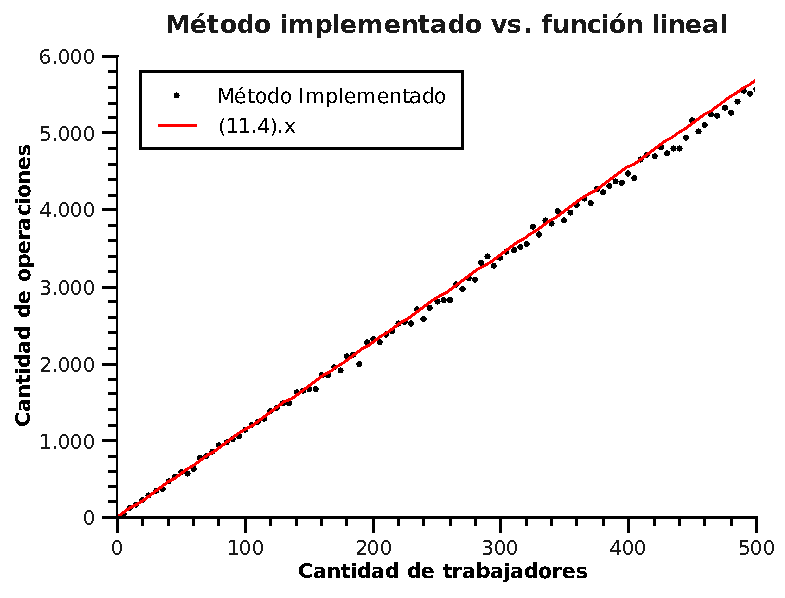
\includegraphics[scale=0.7]{../ej3/graficos/contarOp1.pdf} \\
				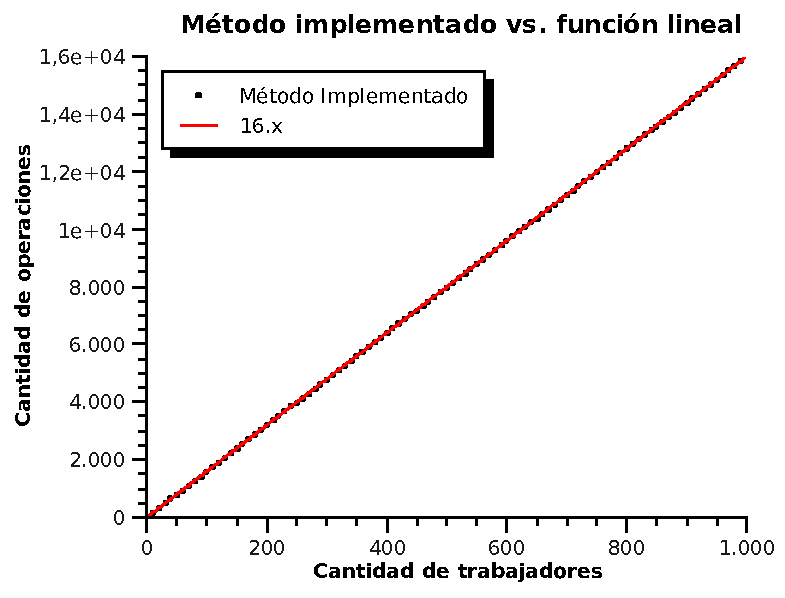
\includegraphics[scale=0.7]{../ej3/graficos/contarOp5.pdf}
				\end{tabular}
				\caption{Muestran el comportamiento de la cantidad de operaciones contra la cantidad de trabajadores. El primer gráfico proviene de una entrada hecha al azar. El segundo proviene de evaluar el comportamiento del algoritmo para el peor caso.} %titulo de la tabla
				\label{cantOpEj3} %con esto puedo referenciar a la tabla \ref{Tiempo metodos}
	\end{table}

	\begin{table}[ht] %ubicacion de la tabla
		\centering %centra la tabla
			\begin{tabular}{c}
				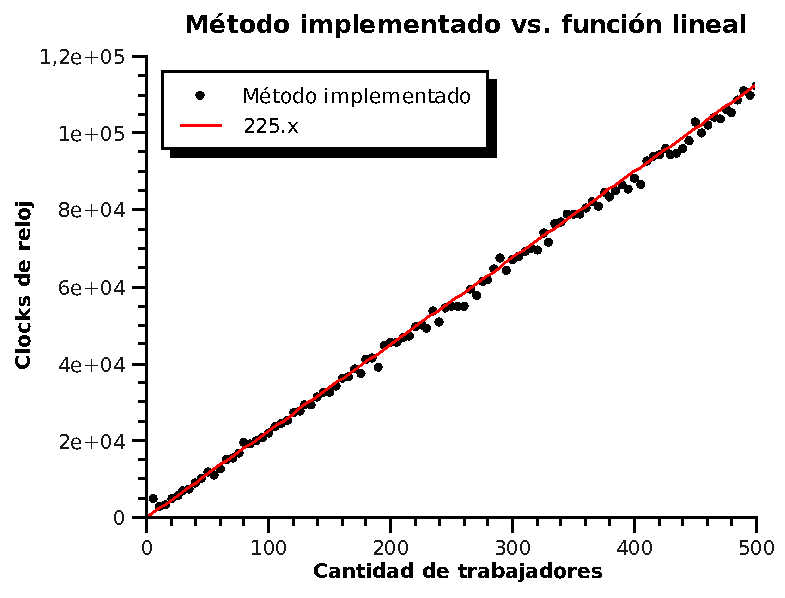
\includegraphics[scale=0.7]{../ej3/graficos/clocks1.pdf} \\
				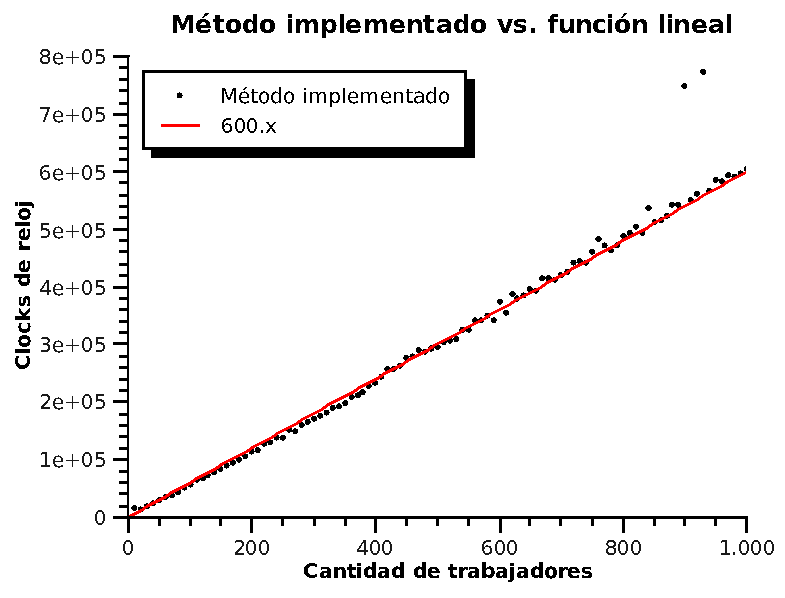
\includegraphics[scale=0.7]{../ej3/graficos/clocks5.pdf}
			\end{tabular}
			\caption{Muestran el comportamiento de la cantidad de ticks de reloj contra la cantidad de trabajadores. El primer gráfico proviene de una entrada hecha al azar. El segundo proviene de evaluar el comportamiento del algoritmo para el peor caso.} %titulo de la tabla
			\label{clocksEj3} %con esto puedo referenciar a la tabla \ref{Tiempo metodos}
	\end{table}

\begin{table}[ht] %ubicacion de la tabla
\centering %centra la tabla
\begin{tabular}{c}
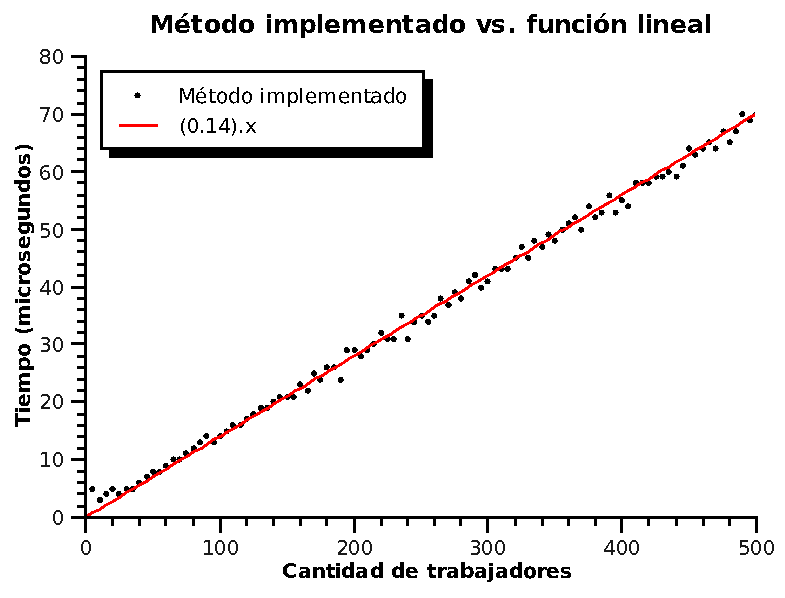
\includegraphics[scale=0.7]{../ej3/graficos/tiempo1.pdf} \\
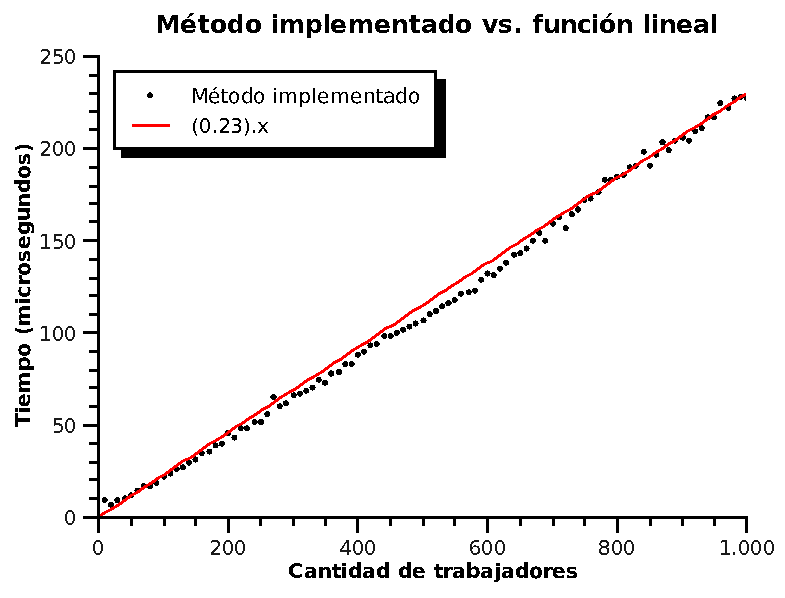
\includegraphics[scale=0.7]{../ej3/graficos/tiempo5.pdf}
\end{tabular}

\caption{Muestran el comportamiento de la cantidad de microsegundos contra la cantidad de trabajadores. El primer gráfico proviene de una entrada hecha al azar. El segundo proviene de evaluar el comportamiento del algoritmo para el peor caso.} %titulo de la tabla
\label{tiempoEj3} %con esto puedo referenciar a la tabla \ref{Tiempo metodos}
\end{table}


\subsection{Debate}
\paragraph{}
Como podemos observar en los gráficos propuestos en la sección [\ref{resultadosej3}] en general la implementación realizada se comporta como se esperaba que en teoría lo hiciera. Es decir, durante el desarrollo del informe sobre este ejercicio, entre otras cosas, hicimos notar que nuestra hipótesis sobre la complejidad del algoritmo era que el mismo tenía un costo de \titade{n}, donde $n$ es la cantidad de trabajadores de la empresa.

\paragraph{}
Se puede identificar en cada gráfico una marcada similitud entre los resultados arrojados en las distintas mediciones que se hicieron sobre la implementación y alguna recta (o función lineal), variando esta última su pendiente para cada caso. Esta pendiente podría compararse o considerarse como la constante que acompa\~na a la complejidad del algoritmo.

\paragraph{}
Se puede notar claramente que esta constante o pendiente, es mayor en aquellos gráficos en los cuales se evaluó el comportamiento del algoritmo en el peor caso que en los que se evaluó el mismo con entradas al azar.

\paragraph{}
En el segundo gráfico perteneciente al cuadro [\ref{clocksEj3}] podemos notar dos casos de outliers. Si observamos más detalladamente se aprecia que estos casos se dan con valores de $n$ grandes. Esto puede deberse a que, como el algoritmo tarda más en terminar\footnote{recordar además que este gráfico corresponde al análisis en el peor caso}, es más probable que haya alguna interrupción que irrumpa durante el procesamiento del mismo haciendo que la medición no sea precisa. Esto se debe a la forma en que se miden los ciclos de reloj. Lo que se hace es obtener los ciclos de reloj transcurridos hasta antes de hacer la llamada al algoritmo implementado, luego se toma la misma medición y, finalmente, se toma la diferencia entre ambas obteniendo como resultado la cantidad de ciclos insumidos por el algoritmo. Pero si durante el algoritmo, llega una interrupción y la atención de la rutina de la misma le insume al procesador varias instrucciones, esto puede llegar a provocar una medición de ciclos de reloj muy imprecisa.\\
Más aún, si tomamos en cuenta cómo un sistema operativo hace manejo de los procesos, puede haber llegado a ocurrir que durante la ejecución del algoritmo, este haya consumido todo su tiempo de ejecución asignado por el sistema, por lo que puede haber tenido que esperar una o incluso varias veces a que el sistema deje continuar con su ejecución.


\subsection{Conclusiones}
\paragraph{}
Luego de describir el funcionamiento del algoritmo, de realizar las pruebas y gráficos pertinentes y de analizarlos detalladamente, podemos realizar algunas conclusiones.\\
Podemos asegurar fehacientemente que la complejidad del algoritmo propuesto es lineal y que la misma es \titade{n} donde $n$ es la cantidad de trabajadores. Esto no sólo se desprende del análisis teórico realizado anteriormente, sino también de las sucesivas pruebas realizadas. Claramente se puede observar en todos los gráficos presentados cómo el comportamiento de la implementación se asemeja a una función lineal sobre los datos de entrada.

\paragraph{}
Finalmente, si hacemos una comparación entre los resultados obtenidos al aplicarse el algoritmo sobre datos de entrada azarosos y datos de entrada que se condicen con el peor caso, se puede observar que la constante que acompaña a la complejidad para el peor caso es considerablemente mayor a la constante que aparece en el caso azaroso. Como una conclusión poco menos significativa entonces, se puede decir que los casos en que los horarios de los trabajadores son todos disjuntos son los peores casos para este algoritmo.
